
\chapter{Hybrid Finite/Boundary Element Method}
\label{sec:hybr-finit-elem}
The hybrid finite/boundary element method works similarly to the normal finite element method except that one or more sub-regions are mapped onto their boundary \cite{Rammohan2002}.
The main advantage of this is that we reduce the dimensionality of these sub-regions one since we only have to solve equations on the boundary instead of the entire space.
In our case this is likely to give an advantage over a pure finite element method since we no longer need to mesh a long way outside the magnetic domain to accurately account for the effect of the external region. Also other methods for dealing with infinite domains can often give additional errors due to the truncation of the external domain.\cite{Bottauscio2008}

On the downside this mapping typically results in a dense matrix after discretisation, to which we cannot apply sparse matrix techniques.
Also the integrals that need to be computed may involve singularities, which introduce additional complications and may reduce accuracy or increase computation time.

Note that the derivation for this hybrid method comes from potential theory, rather than the boundary integral formulation usually used to construct the standard boundary element method.

\section{Derivation of the continuous problem}
\label{sec:bem-derivation}

\subsection{Background of the Method}
\label{sec:basic-method}
We want to use the boundary element method in the calculation of the magnetostatic scalar potential $\phim$, ($\hms = - \nabla \phim$), in the infinite region outside of a magnetic body.
Using the boundary element method directly, however, would require the solution of dense matrix equations for the entire problem.

We can circumvent this problem by splitting the potential into two parts $\phim = \phione + \phitwo$ in such a way that $\phione$ can be calculated the magnetic region(s) using only the finite element method.
We then have some conditions on $\phitwo$ that must be satisfied to give the correct total potential in $\magd$ and on $\boundd$, but, in order to solve for $\phitwo$ in the magnetic domain, we still need to find the boundary conditions (on the edge of the magnetic domain).
So we choose a charge distribution on the boundary that satisfies all the conditions on $\phione$ and $\phitwo$.
We can then solve for $\phitwo$ on the boundary using similar techniques to those used in the boundary element method.
Finally we apply the finite element method to find $\phitwo$ inside the magnetic region $\magd$.

By the uniqueness of solution for Poisson's equation with Dirichlet and/or Neumann boundary conditions we know that the field $ \hms = \nabla \phim$  constructed by the above steps is \emph{the} magnetostatic field.\footnote{To see this take the difference of two solutions of Poisson's equation: $\phi = \psi_1 - \psi_2$. Then using identity \eqref{eq:20}, the linearity of Poisson's equation and the divergence theorem we obtain $\int_S \phi \nabla \phi \cdot d \mathbf{S} = \int_V (\nabla \phi)^2 dV$. Applying Dirichlet, Neumann or mixed boundary conditions shows that the boundary integral is zero and hence $\nabla \phi = 0$.}

\subsection{Problem Description}
\label{sec:problem-description}
Let $\phim^\inte$ be the value of $\phim$ (with subscripts as appropriate) close to the boundary $\boundd$ and just inside the magnetic domain  and $\phim^\exte$ the value of $\phim$ just outside the magnetic domain\footnote{More precisely $\phim^\inte(\xv) = \lim_{\xv \rightarrow \boundd} \phim(\xv)$ from inside the magnetic domain, $\phim^\exte(\xv) = \lim_{\xv \rightarrow \boundd} \phim(\xv)$ from outside the magnetic domain.} (see \autoref{fig:BEM-geometry}).

We have the following \emph{physical} conditions\footnote{Equations~\eqref{eq:2}-\eqref{eqn:phibound} come from the definition of $\phim$, requirement for finite total energy, $\Bv^\text{int} \cdot \nv = \Bv^\text{ext} \cdot \nv$ and ??ds respectively.} on the total magnetostatic potential $\phim$:
\begin{equation}
  \lap \phim(\xv) = \nabla \cdot \mv(\xv) \qquad \forall \xv \in \magd \cup \extd,
  \label{eq:2}
\end{equation}
\begin{equation}
  \phim(\xv) \rightarrow 0 \qquad \text{ as } \abs{\xv} \rightarrow \infty,
\end{equation}
\begin{equation}
  \pd{\phim^\inte(\xv)}{\nv} - \pd{\phim^\exte(\xv)}{\nv} = \mv \cdot \nv \qquad \xv \in \boundd,
  \label{eqn:dphibound}
\end{equation}
\begin{equation}
  \phim^\inte(\xv) - \phim^\exte(\xv)  = 0 \qquad \xv \in \boundd.
  \label{eqn:phibound}
\end{equation}
Note that equations~\eqref{eqn:dphibound} and \eqref{eqn:phibound} imply continuity but not smoothness of the magnetic potential $\phim$ across $\boundd$. This is due to surface magnetic charges.

We choose $\phione$ to satisfy:
\begin{equation}
  \phim(\xv) = \phione(\xv) + \phitwo(\xv) \qquad \forall \xv \in \fulld,
  \label{eq:21}
\end{equation}
\begin{equation}
  \lap \phione(\xv) = \nabla \cdot \mv(\xv) \qquad \xv \in \magd,
  \label{eq:1}
\end{equation}
\begin{equation}
  \pd{\phione^\inte(\xv)}{\nv} = \mv \cdot \nv \qquad \xv \in \boundd,
  \label{eqn:dphionebound}
\end{equation}
\begin{equation}
  \phione(\xv) = 0 \qquad \xv \in \extd.
  \label{eqn:phioneoutside}
\end{equation}
Note that equations~\eqref{eq:1} and \eqref{eqn:dphionebound} give a self contained Poisson Neumann problem for $\phione \in \magd \cup \boundd$.

The equations~\eqref{eq:2} to \eqref{eqn:phibound} for $\phim$ combined with equations~\eqref{eq:21} to \eqref{eqn:phioneoutside} for $\phione$ give a number of conditions on $\phitwo$ must satisfy. Since the Laplacian operator is linear, \ie $\lap \phim = \lap \phione + \lap \phitwo$, from \eqref{eq:2} and \eqref{eq:1} it follows that
\begin{equation}
  \label{eq:8}
  \lap \phitwo(\xv) = 0 \qquad \forall \xv \in \fulld.
\end{equation}

Equation~\eqref{eqn:phioneoutside} implies that $\pd{\phione^\exte(\xv)}{\nv} = 0$. Combining this with equations \eqref{eqn:dphionebound} and \eqref{eqn:dphibound} gives
\begin{equation}
  \label{eq:5}
  \pd{\phitwo^\inte(\xv)}{\nv} - \pd{\phitwo^\exte(\xv)}{\nv} = 0.
\end{equation}

Finally from equations \eqref{eqn:phibound}, \eqref{eq:21} and \eqref{eqn:phioneoutside} we have
\begin{equation*}
  \phione^\inte - \phione^\exte + \phitwo^\inte - \phitwo^\exte = 0,
\end{equation*}
\begin{equation}
  \phitwo^\inte - \phitwo^\exte = - \phione^\inte.
\label{eq:4}
\end{equation}

\begin{figure}
  \center
  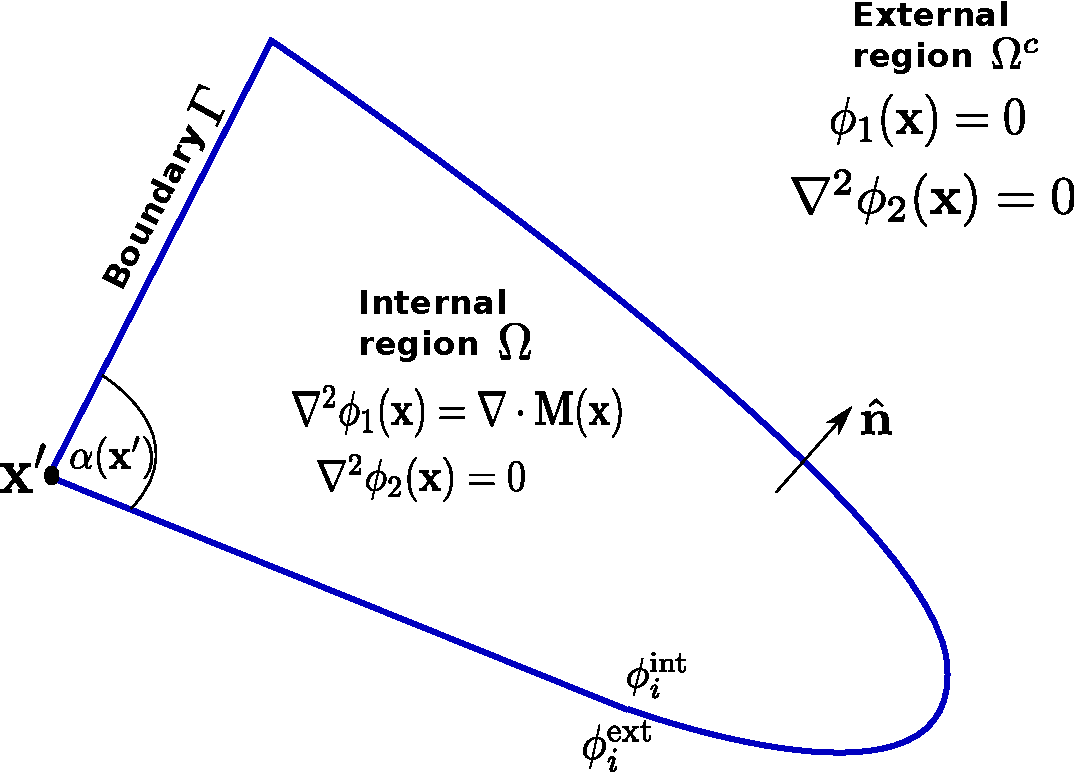
\includegraphics[width=0.75\textwidth]{./images/BEM-geometry}
  % \begin{tikzpicture}

  %   % Main nodes and some labels
  %   \node[label=below:$\xv'$] (a) at (-2,-2) {};
  %   \node (b) at (-2,2) {};
  %   \node[label=right:\Large{$\boundd$}] (c) at (5,0) {};

  %   % Draw main shape of magnetic domain
  %   \draw [line width=0.5mm,draw=solidblue,fill=paleblue] (a.north) to [bend right=71] (c) to (b.south);
  %   \draw [line width=0.5mm,draw=solidblue] (a) to (b);
  %   \draw (a.north) circle(1mm) [fill=black] {};

  %   % More labels
  %   \node (center) at (1,0) {\Large{Magnetic domain $\magd$}};
  %   \node(external) at (8,3) {\Large{External region $\extd$}};
  % \end{tikzpicture}

  \caption{A 2D representation of the geometry showing the labels used in this section. The point $\xv'$ is a singular point of the boundary $\boundd$, the angle $\alpha(\xv')$ is as shown.}
  \label{fig:BEM-geometry}
\end{figure}

\subsection{Double Layer Potentials}
\label{sec:double-layer-potent}
A double layer potential can be thought of as the potential due to a layer of dipoles of magnitude $\mu(\xv)$ in direction $\nv$ over the surface $S$.\cite{Sternberg1946} We will demonstrate that we can use a double layer potential to calculate $\phitwo^\inte$ in terms of $\phione^\inte$.

The double layer potential at a point $\xv \in \real^d$ is defined as \cite{eom_double_layer_potential}
\begin{equation}
  \label{eq:3}
  \phim(\xv) = \int_{S} \mu(\yv) \pd{\Green}{\nv(\yv)} \d \yv,
\end{equation}
where $G$ is the Green's function for a Laplacian operator.
For $d=2$
\[ \Green = \dfrac{-1}{2\pi}\ln(\abs{\xv - \yv}), \]
and for $d=3$
\begin{equation} \Green = \dfrac{-1}{4 \pi} \dfrac{1}{\abs{\xv - \yv}}.
  \label{eqn:greenslaplacian3d}
\end{equation}


We have the following results from potential theory:\cite{Sternberg1946}
\begin{enumerate}
\item The double layer potential satisfies Laplace's equation $\lap \phi = 0$ (in other words the double layer potential is harmonic).% pages ?

\item The double layer potential undergoes a jump of $\mu(\xv)$ moving in the direction $\nv$ across a smooth surface $S$, \ie
  \begin{equation}
    \label{eq:15}
    \phim^\inte(\xv) - \phim^\exte(\xv) = \mu(\xv).
  \end{equation}
% pages 136-140

\item For $\xv \in S$ the following relationship holds
  \begin{equation}
    \phim^\inte(\xv) = (1 - \frac{\alpha(\xv)}{\alpha_{\text{max}}}) \mu(\xv) + \phim(\xv),
    \label{eq:22}
  \end{equation}
  where $\alpha(\xv)$ is the angle (or solid angle) in two (or three) dimensions subtended by the domain at $\xv$ and
\begin{equation*}
  \alpha_{\text{max}} =
  \begin{cases}
    2 \pi & \text{if } d=2 \\
    4 \pi & \text{if } d=3.
  \end{cases}\label{eq:16}
\end{equation*}
Note that $\alpha(\xv)$ is the angle at the exact point $\xv$, when the surface at $\xv$ is a Lyapunov surface (\ie not a sharp corner) $\frac{\alpha(\xv)}{\alpha_{\text{max}}}$ reduces to a factor of $1/2$. We write $\gamma(\xv) = \frac{\alpha(\xv)}{\alpha_{\text{max}}}$ for simplicity.
 % pages 137-139, page 155 for 2d

\item If $\mu$ is continuous and has continuous first and second derivatives along the boundary (\ie $\mu(\xv) \in C^2[S]$) then the limits $\pd{\phim^\inte(\xv)}{\nv}$ and $\pd{\phim^\exte(\xv)}{\nv}$ exist and are equal. % pages 145-153.

\end{enumerate}

Some notes on the derivation of the above results in Sternberg 1946\cite{Sternberg1946}:
\begin{itemize}
\item Some derivations of the results above rely on the surface being a ``Lyapunov surface'' which imposes a number of smoothness conditions, in particular excluding surfaces with corners.
The proofs given in Sternberg allow a finite number of sharp corners, \ie a polygonal domain.
\item Our potentials are a factor of $\frac{-1}{4 \pi}$ different from those in the reference. Also our $\phim^\inte$ and $\phim^\exte$ definitions correspond respectively to $\phim^-$ and $\phim^+$ in the book.
\end{itemize}

\subsection{Application to Magnetostatic Calculations}
\label{sec:appl-magn-calc}

From \autoref{sec:double-layer-potent} we can see that conditions \eqref{eq:8}, \eqref{eq:5} and \eqref{eq:4} on $\phitwo$ are satisfied by a double layer potential with magnitude
\begin{equation}
  \label{eq:24}
  \mu(\xv) = - \phione^\inte(\xv).
\end{equation}

By the uniqueness of solution for Poisson's equation this gives us, up to an additive constant, the only solution for $\phitwo(\xv)$ in the external region.
This is good enough for a potential since it is only used in $\hms(\xv) = - \nabla \phim(\xv)$ so addition of a constant has no effect.

From equations~\eqref{eq:3}, \eqref{eq:22} and \eqref{eq:24} we have:
\begin{equation}
  \label{eq:6}
  \phitwo^\inte(\xv) =  \big(\gamma(\xv) - 1 \big) \phione^\inte(\xv)
  - \int_{\boundd} \phione^\inte(\yv) \pd{\Green}{\nv(\yv)} \d \yv.
\end{equation}
After substituting in our definition for the three dimensional Green's function \eqref{eqn:greenslaplacian3d} we obtain the same equation as given by Koehler \cite{Koehler1997}.
Similar equations are solved when using the standard boundary element method, hence the name.

Also note that $\phim = \phione + \phitwo$ everywhere and so
\begin{align}
  \label{eq:18}
  \phim^\inte(\xv) &= \bm \big[ \phione^\inte(\xv) \big] \\
  &= \gamma(\xv) \phione^\inte(\xv)
  - \int_{\boundd} \phione^\inte(\yv) \pd{\Green}{\nv(\yv)} \d \yv. \notag
\end{align}

Either equation~\eqref{eq:6} or \eqref{eq:18} can be used to give boundary conditions for $\phitwo \in \magd$ or $\phim \in \magd$ respectively. We will proceed using equation~\eqref{eq:18} for simplicity since it eliminates $\phitwo$ from later calculations.

Hence, given the solution for $\mv(\xv) \in \magd$ the complete continuous problem is
 \begin{subequations}
   \label{eq:phi-bem-continuous}
   \begin{align}
     \label{eq:phim-bem-continuous}
     \lap \phim(\xv) &= \div \mv(\xv) \quad & \xv \in \magd, \\
     \label{eq:phi1-bem-continuous}
     \lap \phione(\xv) &= \div \mv(\xv)    & \xv \in \magd,
   \end{align}
 \end{subequations}
with boundary conditions
 \begin{subequations}
   \label{eq:phi-bem-continuous-bc}
   \begin{align}
     \label{eq:phim-bem-continuous-bc}
     \phim(\xv) &= \bm \big[ \phione(\xv) \big]      & \xv \in \boundd, \\
     \label{eq:phi1-bem-continuous-bc}
       \pd{\phione(\xv)}{\nv} &= \mv \cdot \nv  & \xv \in \boundd.
   \end{align}
 \end{subequations}
Here we have dropped the distinction between $\inte$ and $\exte$ since all exterior values have been eliminated.


\section{Discretisation}
\label{sec:discretisation}

The bulk equations~\eqref{eq:phi-bem-continuous} and the boundary condition on $\phione$, equation~\eqref{eq:phi1-bem-continuous-bc}, are identical to those discussed in \autoref{sec:magn-field-resid}.
As such the weak residual form, discretisation and Jacobian calculations are identical for these equations.
Therefore all that remains to be discretised is the operator $\bm$. We let
\begin{equation}
  \phim = \sum_\ibasis \phim_{\ibasis} \tbf_{\text{m},\ibasis}(\xv),
  \qquad
  \phione = \sum_\ibasisb \phione_{\ibasisb} \tbf_{1,\ibasisb}(\xv),
  \label{eq:25}
\end{equation}
where $\tbf_\ibasis(\xv_\ibasisb) = \delta_{\ibasis \ibasisb}$ on the boundary nodes and is linearly interpolated from $\tbf_\ibasis = 1$ at $\xv_\ibasis$ to $\tbf_\ibasis = 0$ at neighbouring nodes.

Substituting equations~\eqref{eq:25} into \eqref{eq:18} we have
\begin{equation*}
  \sum_\ibasis \phim_{\ibasis} \tbf_{\text{m},\ibasis}(\xv) =
  - \int_{\boundd} \sum_\ibasisb \phione_{\ibasisb} \tbf_{1,\ibasisb}(\yv)
  \pd{\Green}{\nv(\yv)} \d \yv
  \quad + \gamma(\xv) \sum_\ibasisb \phione_{\ibasisb} \tbf_{1,\ibasisb}(\xv).
\end{equation*}

To get the value of $\phim$ at node $\ibasisc$ we choose $\xv = \xv_\ibasisc$. Then using the property $\tbf_\ibasis(\xv_\ibasisc) = \delta_{\ibasis \ibasisc}$ and replacing $\ibasisc$ by $\ibasis$ we have
\begin{equation}
  \phim_{\ibasis} =
  - \int_{\boundd_\ibasisb} \sum_\ibasisb \phione_{\ibasisb} \tbf_{1,\ibasisb}(\yv)
  \pd{\Green[\ibasis]}{\nv(\yv)} \d \yv
  \quad + \gamma(\xv_\ibasis) \phione_{\ibasis},
  \label{eq:colocation}
\end{equation}
where ${\boundd_\ibasisb}$ is the region where $\tbf_{1,\ibasisb} \neq 0$, \ie the elements which contain node $\ibasisb$.

Finally, since the integrands are continuous functions ??ds citation needed, we can move the sum outside the integral leaving
\begin{equation}
  \phim_{\ibasis} =
  - \sum_\ibasisb \phione_{\ibasisb} \Big[ \int_{\boundd_\ibasisb} \tbf_{1,\ibasisb}(\yv)
  \pd{\Green[\ibasis]}{\nv(\yv)} \d \yv \Big]
  \quad + \gamma(\xv_\ibasis) \phione_{\ibasis}.
\label{eq:27}
\end{equation}
Notice that the expression inside the square brackets is independent of all the potentials: it depends only on the geometry and so can be pre-calculated and stored in many cases.

So equation~\eqref{eq:27} gives $\phim$ at a boundary node in terms of a sum of geometric factors multiplied by $\phione$ at each boundary node.
In other words, this is a dense matrix multiplication by a pre-computed matrix giving $\phim$ at all the boundary nodes in terms of $\phione$ at all boundary nodes:
\begin{equation}
  \label{eq:10}
  \phim_\ibasis = \bm_{\ibasis,\ibasisb} \cdot \phione_{\ibasisb},
\end{equation}
where
\begin{equation}
  \label{eq:17}
  \bm_{\ibasis\ibasisb} = - \int_{\boundd_\ibasisb} \tbf_{1,\ibasisb}(\yv) \pd{\Green[\ibasis]}{\nv(\yv)} \d \yv
  \quad + \gamma(\xv_\ibasis)\delta_{\ibasis\ibasisb}.
\end{equation}


% ??ds wrong place for this discussion and not sure if integral is really singular or not due to the n.r term...
%Note that although this integral appears at first glance to be singular when the node $\xv_\ibasis$ is within $\boundd_\ibasisb$ (the line segment or section of surface being integrated over)
%A benefit of this is that the matrix is always well conditioned because the largest terms are near the singularity and hence near the diagonal elements $\ibasisb = \ibasis$.
%However the singularity can cause difficulties in the evaluation of the affected integrals.
%Methods to overcome these difficulties are discussed in the next section.

We now convert the normal derivative of the Green's function into a more tangible form.
In 3D
\begin{equation}
  \label{eq:11}
  \pd{\Green}{\nv} = \frac{-1}{4 \pi} \pd{}{\nv} \Gthreed = \frac{-1}{4 \pi} \nv \cdot \nabla \Big( \Gthreed \Big).
\end{equation}
Converting to spherical coordinates with the origin at $\xv$ ($r = \abs{\yv - \xv}$, $\ruv = \frac{\yv - \xv}{r}$) we have\footnote{In spherical polar coordinates $\nabla = \ruv \pd{}{r} +  \phiv \frac{1}{r} \pd{}{\phi} + \thetav \frac{1}{r \sin \theta} \pd{}{\theta}$. Obviously $\frac{1}{r}$ has no angular dependence so only the derivative with respect to $r$ is non-zero.}
\begin{equation}
  \label{eq:12}
  \pd{G(r)}{\nv} = \frac{-1}{4 \pi} \nv \cdot \ruv \pd{}{r} \Big( \frac{1}{r} \Big)
  = \frac{+1}{4 \pi}  \frac{\nv \cdot \ruv}{r^2},
\end{equation}
\begin{equation}
  \label{eq:13}
  \pd{\Green}{\nv} = \frac{\nv \cdot (\yv - \xv)}{4 \pi \abs{\yv - \xv} ^2} .
\end{equation}
Similarly in 2D we find
\begin{equation}
  \label{eq:14}
  \pd{\Green}{\nv} = \frac{-1}{2 \pi} \pd{}{\nv} (\Gtwod) = \frac{\nv \cdot (\yv - \xv)}{2 \pi \abs{\yv - \xv}}.
\end{equation}

So the discretised boundary element matrix in $d=2,3$ dimensions is
\begin{equation}
  \label{eq:19}
  \bm_{\ibasis\ibasisb} =\frac{-1}{2^{(d-1)} \pi} \int_{\boundd_\ibasisb} \tbf_{1,\ibasisb}(\yv) \frac{\nv(\yv) \cdot (\yv - \xv_\ibasis)}{\abs{\yv - \xv_\ibasis} ^{d-1}} \d \yv
   \quad + \gamma(\xv_\ibasis)\delta_{\ibasisb\ibasis}.
\end{equation}
We denote the integral in this equation by $I_\bm$.

\subsection{Discretisation Approaches: Co-location vs Galerkin}

In deriving equation~\eqref{eq:colocation} we used a co-location approach rather than the Galerkin approach used in our FEM method.
The reason for this choice is that a Galerkin discretisation would lead to a double integral over the boundary, which would probably be more difficult to calculate.

Not sure what effect this has, if any, on the stability or accuracy of the scheme...

\section{Evaluation of the discrete boundary operator}
\label{sec:calc-integr-i_bm}

\section{Singularity of the main integral}
\label{sec:bem-singularity}

Another factor that should be considered is the apparent singularity in the integral $I_\bm$ when integrating over an element containing the source point $\xv_\ibasis$. There are two distinct cases to look at here: flat elements and curvilinear elements.

In the case of flat elements if $\xv_\ibasisb$ is within the element being integrated over then we have
\begin{equation}
  \label{eq:7}
  \nv(\yv) \cdot \ruv_{\xv_{\ibasis} \rightarrow \yv} \equiv 0 \quad \forall \yv \in \text{element}.
\end{equation}
So the integral is zero and the singularity is avoided. Unfortunately for neighbouring elements this is not necessarily true--in particular elements at a sharp corner may be very close to a node where $\nv(\yv) \cdot \ruv_{\xv_{\ibasis} \rightarrow \yv} \neq 0$ resulting in a near-singular integral.

For curvilinear elements we no longer have the nice property that any potentially singular elements are automatically zero. However it can be shown that for reasonably shaped elements ??ds citation needed! there are still no real singular integrals only near-singular ones. This is due to the fact that $\nv(\yv) \cdot \ruv_{\xv_{\ibasis} \rightarrow \yv}$ tends to zero ``faster'' than $\abs{\yv - \xv_\ibasis}^2$ so the limit of the ratio as $\yv \rightarrow \xv_\ibasis$ is zero. In fact integrals like this are routinely evaluated in standard boundary element methods ??ds citation needed.


\subsection{Corner Singularities}

Have to handle calculation of angles/solid angles $\gamma(\xv)$ somehow.

So far I've just assumed the information will be provided

Inderpretations: only count ``real'' sharp corners (\ie sphere has no corners) vs include all element corners (\ie sphere has sharp corners at every element join).


\subsection{Analytical solutions}

??ds you need to thoroughly check the maths in this section at least once more

For linear shape functions and triangular elements an exact analytical solution for the singular integral $I_G$ was given by Lindholm \cite[App. B]{Lindholm1984}\footnote{Note: Lindholm's definition of the 3d Green's function is a factor of -1 different to ours.}, the original derivation is due to Collie\cite{Collie1976}. 
Combining equations (2) and (3) from \cite{Lindholm1984} with equation~\eqref{eq:13} and using our notation for positions, we see that Lindholm's $L$ operator is
\begin{equation}
  \begin{aligned}
    L[U] &= \frac{-1}{4 \pi}\int_\boundd U(\yv) \frac{\nv(\yv) \cdot (\yv -
      \xv)}{\abs{\xv - \yv}^2}
    \d\yv, \\
    &= -G[U] + \gamma(\xv) U(\xv).
  \end{aligned}
\end{equation}
So $L[\tbf_{1,\ibasisb}]$ integrated over the surface triangle $\boundd_\ibasisb$ with $\xv = \xv_\ibasis$ corresponds exactly to the integral $I_{G,i,j}$ required in the calculation of $G_{i,j}$\footnote{The minus sign from the different definitions of the Green's function has cancelled with the minus sign from the fact that we are interested in calculating $-1$ times the operator.}.

To clearly see the equivalence between the discretised operators we need to go through both discretisations simultaneously.
Ignoring sharp corners we have that
\begin{equation}
  \begin{aligned}
    \phim(\xv) = G[\phione](\xv) &= -L[\phione](\xv), \\
    %
    \sum_{n} \phim_n \tbf_n(\xv) 
    &= - \sum_{\tri=1}^{N_\tri} \sum_{i=1}^{3} L_{\tri,i}(\xv) \phione_{\tri,i}, 
    \quad\quad&\text{expand}\\
    % 
    \sum_{n} \phim_n \tbf_n(\xv) 
    &= - \sum_{\tri=1}^{N_\tri} \sum_n L_{\tri,n}(\xv) \phione_n, 
    &\text{equivalent to sum over all nodes--local support}\\
    % 
    \phim_k &= - \sum_{\tri=1}^{N_\tri} \sum_n L_{\tri,n}(\xv_k) \phione_n, 
    &\text{use $\tbf_n(\xv_k) = \delta_{nk}$}\\
    % 
    \phim_k &= \sum_n \bigs{\sum_{\tri=1}^{N_\tri} -L_{\tri,n}(\xv_k)} \phione_n, 
    &\text{reorder}\\
    %
    \phim_k &= \sum_n \bigs{\sum_{\tri \in \text{around}(n)} -L_{\tri,n}(\xv_k)} \phione_n,
    &\text{reduce elements to sum over--local support again}\\
    %
    &= \sum_n G_{k,n} \phione_n. 
    &\text{equation~\eqref{eq:10}}
  \end{aligned}
\end{equation}
Therefore 
\begin{equation}
  IG_{i,j} = \sum_{\tri \in \text{around}(j)} L_{\tri,k}(\xv_i),
\end{equation}
where $k$ is the index of node $j$ within triangle $\tri$.

Let
\begin{equation}
  \begin{aligned}
    \rv_k(\xv) &= \zv_k - \xv, &\quad \text{(vector from triangle node $k$ to $\xv$)} \\
    \sv_k &= \zv_{k+1} - \zv_k, & \text{(vector along an edge of the triangle)} \\
  \end{aligned}
\end{equation}
and let $\hat{\sv}$, $\hat{\rv}$ be the equivalent unit vectors.
Hence using the third (un-numbered) equation in appendix B of \cite{Lindholm1984}, converting to our notation and substituting in values from the rest of appendix B where practical we have
\begin{equation}
  \begin{aligned}
    \label{eq:analytic-bem-integral}
    I_{G,i,j} &= \sum_{\tri \in \text{around}(j)} \frac{\abs{\sv_{k+1}}}{8 \pi A_\tri} \bigb{
      \bigb{(\nv_\tri \times \hat{\sv}_{k+1}) \cdot \rv_{k+1}(\xv_i)} \Omega_\tri(\xv_i) 
      - \nv_\tri \cdot \rv_1(\xv_i) \sum_{l=1}^{3} (\hat{\sv}_{k+1} \cdot \hat{\sv}_l) P_l(\xv_i)
    }, \\
  \end{aligned}
\end{equation} 
where $A_\tri$ is the area of the triangle, $\zv_i$ denote the nodes of triangle $\tri$ (mod 3), and $\nv_\tri$ is the unit normal to the triangle. 
The quantity $P_l(\xv)$ is given by
\begin{equation}
  P_l(\xv) = \ln\bigb{\frac{\abs{\rv_l(\xv)} + \abs{\rv_{l+1}(\xv)} + \abs{\sv_l}}
    {\abs{\rv_l(\xv)} + \abs{\rv_{l+1}(\xv)} - \abs{\sv_l}}}.
\end{equation}
Finally we need $\Omega_\tri$, the solid angle subtended by the triangle at $\xv_i$:
\begin{equation}
  \label{eq:bem-triangle-solid-angle}
  \Omega_\tri(\xv) = \text{sign}(\nv_\tri \cdot \rv_1) 2 \cos^{-1}\bigs{\frac
    {\abs{\rv_1}\abs{\rv_2}\abs{\rv_3} + \abs{\rv_1} \rv_2\cdot\rv_3 + \abs{\rv_2}\rv_1\cdot \rv_2}
    {\sqrt{2(\abs{\rv_2}\abs{\rv_3} + \rv_2\cdot\rv_3)
        (\abs{\rv_3}\abs{\rv_1} + \rv_3\cdot\rv_1)
        (\abs{\rv_1}\abs{\rv_2} + \rv_1\cdot\rv_2)}}},
\end{equation}
where we have dropped the $\xv$ argument from $\rv_i(\xv)$ for brevity.
The use of $\rv_1(\xv)$ in equations~\eqref{eq:analytic-bem-integral} and \eqref{eq:bem-triangle-solid-angle} is not a typo: the results are independant of which node in the triangle is used.


A useful open source implementation of this calculation in \texttt{C} is included in \texttt{magpar}\cite{magpar-website-dummy} and redistributed in \texttt{nmag}\cite{nmag-website-dummy}.


\subsubsection{Numerical integration}

The analytical formula given in the previous Section is fast and accurate when applicable but also greatly limits the allowed meshes.
It is very useful when testing code to be able to run 2D simulations, since the run time can be orders of magnitude smaller.
It is also sometimes useful to be able to use structured quadrilateral meshes for simple geometries and for testing purposes.
??ds higher order elements?
Both of these approaches are impossible with the analytical formula above.
It is likely that similar analytical results could be derived for each of these cases, but it is simpler and more general to use a numerical approach instead.

As discussed in \autoref{sec:bem-singularity} the integral $I_G$ is non-singular, so no special techniques are needed for its integration (other than what is needed to attain good accuracy).
As such an adaptive quadrature method can effectively calculate the integrals.
Our algorithm is roughly as follows:
\begin{enumerate}
\item Calculate the integral twice with different orders of quadrature.
\item If the difference is less than some tolerance then accept the result.
\item Otherwise repeat the calculation with a higher order quadrature, and goto 2.
\end{enumerate}

Alternate adaptivity process: use h-refinement instead/as well (divide integral into chunks). ??ds did I consider this?

Ideally we would like to include the calculations at lower order quadratures in the higher order ones, therefore use ??ds Clenshaw-Curtis quadrature\cite{Trefethen2008}.

Rapid increase in quadrature order to avoid wasting time calculating many intermediate attempts.

Formulae from ??ds.

Potentially problems could arise when $\xv_i$ is extremely close to the surface element, but not in the same plane (so that $\nv \cdot \rv \neq 0$).
This would occur, for example, in extremely thin or extremely sharp regions of magnetic material.
Such regions are unlikely to be a problem in practice because sufficiently thin/sharp domains are likely to be outside the scope of micromagnetism in general.



\section{Solution of the linear systems}
\label{sec:solution-strategies}

??ds new chapter?

The BEM matrix is dense and so requires some tricks/discussion.

Two ways to proceed with solving the coupled system of equations~\eqref{eqn:ndllg-starting}, \eqref{eq:phi-bem-continuous-bc} and \eqref{eq:phi-bem-continuous-bc}.
First is to solve the entire system as a single non-linear pde.
Second is to make the assumption that magnetostatic field part is non-stiff and solve semi-implicitly as two sets of coupled pdes.
Each method has its own advantages.


\subsection{The Matrix $\bm$}

Since $\bm$ is a dense matrix the processing and memeory requirements to compute, store and use $\bm$ scales as $\order{N_b^2}$ where $N_b$ is the number of boundary nodes. For some geometries (\eg nearly spherical objects) the overall computational complexity remains $\order{N}$ but for others (especially very thin films) the complexity can approach $\order{N^2}$.

It should be noted that $\bm$ depends only on the geometry of the problem and so typically only needs to be computed once, at the beginning of the simulation. Hence the integral computation time is not too important. Although if spatial adaptivity is used the geometry will change with every adaptation and $\bm$ will need to be recalculated.

One way to reduce the problems associated with the dense nature of $\bm$ is to use hierarchical matrix techniques. In this type of matrix the less important entries (\ie smaller) are lumped into a single entry similarly to multipole approximation methods. The cost of multiplication and storage of $\bm$ is thus reduced to only $\order{N \log(N)}$.\cite{Knittel2009}


\subsection{Fully implicit}

??ds mention TR blows up with semi-implicit + numerical experiments

Solve the entire system as one coupled non-linear pde.
This means that we are using a well understood time integration scheme rather than some relatively unknown approximation.
The downside is that the Jacobian will contain the dense matrix $\bm$, which makes solving the system in a naive manner extremely expensive.
In this section we will discuss solvers which can make this process comparatively efficient.

Another advantage of this method over the semi-implicit method arises when using IMR.
The energy conservation property of IMR is the most unique of its geometrical integration properties\footnote{A number of explicit integration schemes can obtain length conservation: Cayley transform methods\cite{Lewis2003}, semi-analytical methods\cite{Wiele2010} and various types of semi-implicit midpoint rule methods\cite{Spargo2003a}\cite{Mentink2010} (including the one described in this section).}, but it is lost when a semi-implicit method is used.

To enforce the Dirichlet boundary condition within the Newton solver we use the slightly odd residual
\newcommand{\rphimb}{\rphi_b}
\begin{equation}
  \rphimb(\phim_b, \phione_b) = \bm[\phione_b] - \phim_b.
\end{equation}
Everything else proceeds as normal.


\subsubsection{Jacobian structure}
\label{sec:bem-jacobian-structure}

As mentioned in \autoref{sec:discretisation} the pair of Poisson equations for the FEM/BEM method are essentially the same as those in \autoref{sec:galerk-meth-llg}.
The first difference is that there is no coupling from the auxilary potential $\phione$ to the LLG equations, and hence no corresponding $\Pm$ block.
The second difference is that there is an additional coupling between the boundary values of the auxilary potential and the boundary values of the real potential $\phim$.

With the order of blocks as: $\mv$, $\phim$, $\phione$, $\phione$ boundary.
Then the Jacobian is
\begin{equation}
  \Jm = 
  \begin{pmatrix}
    \Fm       & \Pm     &  \\
    \Qm'      & \Am' &  \bm'  \\
    \Qm       &         &   \Am
  \end{pmatrix},
\end{equation}

%% all in one:
% \begin{equation}
%   \Jm = 
%   \begin{pmatrix}
%     \Fm       & \Pm     & \Pm_b  &         &           \\
%     \Qm       & \Am     & \pd{\phim}{\phim_b}  &         &           \\
%     &         & -\Idm  &         &  \bm      \\
%     \Qm       &         &        & \Am     & \pd{\phione}{\phione_b}   \\
%     \Qm_b     &         &        & \pd{\phione_b}{\phione} & \Am_b      
%   \end{pmatrix}
% \end{equation}

where the primed blocks are ones where the boundary and bulk values must be split up because of the BEM boundary condition.
So
\begin{equation}
  \Am' =
  \begin{pmatrix}
     \Am     & \pd{\phim}{\phim_b} \\
       0      & -\Idm  
  \end{pmatrix},
\end{equation}
\begin{equation}
  \Qm' =
  \begin{pmatrix}
    \Qm \\
    0    
  \end{pmatrix},
\end{equation}
and
\begin{equation}
  \bm' =
  \begin{pmatrix}
     0  & 0 \\
     0  & \bm 
  \end{pmatrix}.
\end{equation}


It is worth noting that a slightly different Jacobian struture could be obtained by modifying the derivation in \autoref{sec:appl-magn-calc}.
Instead of using $\phim = \phione + \phitwo$ to eliminate $\phitwo$, we could have written $\hms = - \grad \phione - \grad \phitwo$.
This would result in both of the potentials having a $\Pm$ block, but only one of them having a $\Qm$ block.
It would also reduce the diagonal dominance of $\bm$, which is probably a bad thing ??ds check? are we sure?


\subsubsection{Solver strategies}
\label{sec:bem-solver-strategies}

The first technique for an efficient strategy is to use a hierarchical matrix representation for $\bm$.
This greatly increases the asymptotic efficiency of operations, for example multiplication only takes $\order{N_b \log N_b}$ instead of $\order{N_b^2}$ time where $N_b$ is the number of boundary nodes.
However this rules out the use of a straightforward direct solver.
Hence we need to use some form of block-wise solver where it is possible to treat seperate blocks differently.
A simple way to do this is to use a Krylov subspace method.
In such a solver all that is needed is a way to calculate matrix-vector products for $J$, which can easily be done in a block-wise manner.

\newcommand{\prcd}{\mathcal{P}}

First preconditioner: exact solve w/out $\bm$.
\begin{equation}
  \prcd_{1} = 
  \begin{pmatrix}
    \Fm       & \Pm     &  \\
    \Qm'       & \Am'    &   \\
    \Qm       &         &   \Am
  \end{pmatrix}.
\end{equation}

Second preconditioner: block triangular with AMG, exact LLG blocks, drop $\Pm$ and $\bm$.
\begin{equation}
  \prcd_{2} = 
  \begin{pmatrix}
    \Fm       &           &  \\
    \Qm'       & \hat{\Am'}&   \\
    \Qm       &           &   \hat{\Am}
  \end{pmatrix}.
\end{equation}

Third preconditioner: nested block triangular with AMG, exact LLG blocks, drop $\Qm$ and $\bm$,
\begin{equation}
  \prcd_{2} = 
  \begin{pmatrix}
    \Fm       & \Pm       &  \\
              & \hat{\Am'}&   \\
    \Qm       &           &   \hat{\Am}
  \end{pmatrix}.
\end{equation}
Use a nested block triangular preconditioner rather than reordering to avoid having varying Jacobian orders.

Q is a much simpler block (linear, only one term) so probably best to drop that?

??ds try exact A for each of these?


\subsection{Semi-implicit}
\label{sec:semi-implicit-bem}

The alternative to a fully implicit solve is to come up with a semi implicit method.
The idea is to approximate $\phim$ using an explicit time integration method while still using an implicit method for $\mv$.
This means that the system no longer has the properties of the purely implicit method.
We hope that despite this it will retain sufficient stability to allow long time steps.

The strategy is as follows:
\begin{enumerate}
\item Calculate $\phim_0$ from initial condition $\mv_0$.
\item Extrapolate $\phim_n$ to $t_{n+1}$ using a second order formula to get $\hat{\phim}_{n+1}$.
\item Use $\hat{\phim}_{n+1}$ to calculate $\mv_{n+1}$ (implicitly in $\mv_{n+1}$).
\item Calculate $\phione_{n+1}$ using $\mv_{n+1}$.
\item Use boundary values of $\phione_{n+1}$ to get $\phim_{n+1}$.
\item If not finished then goto 2.
\end{enumerate}

A simple second order extrapolation formula (based on Lagrange interpolation\cite[312]{Kincaid2002}) is 
\begin{equation}
  \label{eq:65}
  f(t) = \frac{t - t_1}{t_0 - t_1}f(t_0) + \frac{t - t_0}{t_1 - t_0}f(t_1).
\end{equation}
After substituting in $t=t_{n+1}$, $t_1=t_n$ and $t_0=t_{n-1}$ this gives an expression for the predicted $\phim$ value
\begin{equation}
  \label{eq:66}
  \hat{\phim}_{n+1} = \frac{-\dtx{n+1}}{\dtn} \phim_{n-1} + \frac{\dtx{n+1} + \dtn}{\dtn} \phim_n.
\end{equation}

Note that if we are using the implicit midpoint rule then we actually want to extrapolate $\phim$ to the midpoint, hence we actually use $\dtx{n+1} = \dtx{n+1} /2$ in the above equation.
If we are using the implicit midpoint rule with constant time steps then the extrapolation formula becomes
\begin{equation}
  \label{eq:67}
  \hat{\phim}_{n+1} = \frac{1}{2} \phim_{n-1} + \frac{3}{2} \phim_n,
\end{equation}
which matches with the extrapolation formula given for a different semi-implicit version of the midpoint rule\cite{Serpico2001}.

Notes:
\begin{itemize}
\item stability uncertain: polynomial extrapolation can be dodgy..
\item Need to find error expression for extrapolation
\item talk about relation to FEM (Lagrange polynomials)?
\end{itemize}

\subsubsection{Jacobian structure}
\label{sec:bem-jacobian-structure}

Decoupling the system as discussed above means that we only need to solve the LLG system (as discussed in \autoref{sec:llg-jacobian}) along with two Poisson systems of size $\sim N$ (as given in \autoref{sec:poisson-jacobian}).
Additionally we need to perform a single matrix multiply (of size $N_b$) to calculate the boundary conditions on the $\phim$ Poisson solve.


\subsubsection{Solver strategies}
\label{sec:semi-implicit-bem-solver-strategies}

As discussed above we use a hierarchical matrix representation for the BEM operator $\bm$, to avoid large memory requirements and to speed up the dense matrix multiply.

Efficient solver strategies for Poisson systems are extremely well studied.
An efficent and robust method for solving Poisson systems on unstructured grids is to use the method of conjugate gradients with a single V-cycle of algebraic multigrid as a preconditioner \cite[Chap. 2]{HowardElmanDavidSilvester2006}.

Solver strategies for the LLG system are discussed in \autoref{??ds llg preconditioning}.


%%% Local Variables:
%%% mode: Latex
%%% TeX-master: "main"
%%% End:
